%{{{ Formatierung

\documentclass[a4paper,10pt]{article}

\usepackage{physics_notetaking}

%%% dark red
%\definecolor{bg}{RGB}{60,47,47}
%\definecolor{fg}{RGB}{255,244,230}
%%% space grey
%\definecolor{bg}{RGB}{46,52,64}
%\definecolor{fg}{RGB}{216,222,233}
%%% purple
%\definecolor{bg}{RGB}{69,0,128}
%\definecolor{fg}{RGB}{237,237,222}
%\pagecolor{bg}
%\color{fg}

\newcommand{\td}{\,\text{d}}
\newcommand{\RN}[1]{\uppercase\expandafter{\romannumeral#1}}
\newcommand{\zz}{\mathrm{Z\kern-.3em\raise-0.5ex\hbox{Z} }}
\newcommand{\id}{1\kern-.258em1}

\newcommand\inlineeqno{\stepcounter{equation}\ {(\theequation)}}
\newcommand\inlineeqnoa{(\theequation.\text{a})}
\newcommand\inlineeqnob{(\theequation.\text{b})}
\newcommand\inlineeqnoc{(\theequation.\text{c})}

\newcommand\inlineeqnowo{\stepcounter{equation}\ {(\theequation)}}
\newcommand\inlineeqnowoa{\theequation.\text{a}}
\newcommand\inlineeqnowob{\theequation.\text{b}}
\newcommand\inlineeqnowoc{\theequation.\text{c}}

\renewcommand{\refname}{Source}
\renewcommand{\sfdefault}{phv}
%\renewcommand*\contentsname{Contents}

\newenvironment{Figure}
        {\par\medskip\noindent\minipage{\linewidth}}
        {\endminipage\par\medskip}

\pagestyle{fancy}

\sloppy

\numberwithin{equation}{section}

%}}}

\begin{document}

%{{{ Titelseite

\begin{titlepage}
	\title{5 (1.\ Halbtag) $|$ Operationsverstärker}
	\author[1]{Angelo Brade\thanks{s72abrad@uni-bonn.de}}
	\author[1]{Jonas Wortmann\thanks{s02jwort@uni-bonn.de}}
	\affil[1]{Rheinische Friedrich--Wilhelms--Universität Bonn}
	\date{\today}
\end{titlepage}

\maketitle
\pagenumbering{gobble}

%}}}

\newpage

%{{{ Inhaltsverzeichnis

\fancyhead[R]{\leftmark}
%\fancyhead[R]{\leftmark\\\rightmark}
\fancyhead[L]{\thepage}
\fancyfoot[C]{}

\tableofcontents

%}}}

\clearpage

%{{{

\pagenumbering{arabic}

\begin{multicols}{2}

	\section{Introduction}
	This experiment deals with the opamp and its funcitonality in different circuits.
	The opamp can be used as a non--inverting or inverting amplifier, adder, differential amplifier, current source, monoflop, to logarithmize or exponentiate and to differentiate or integrate a signal.
	It is also possible to build a \textsc{Schmitt}--trigger or an astable multivibrator.
	In this experiment the opamp will serve as a non--inverting amplifier, adder, current source, integrator and differential amplifier.

	\section{Theory}
	\begin{Figure}
		\centering
		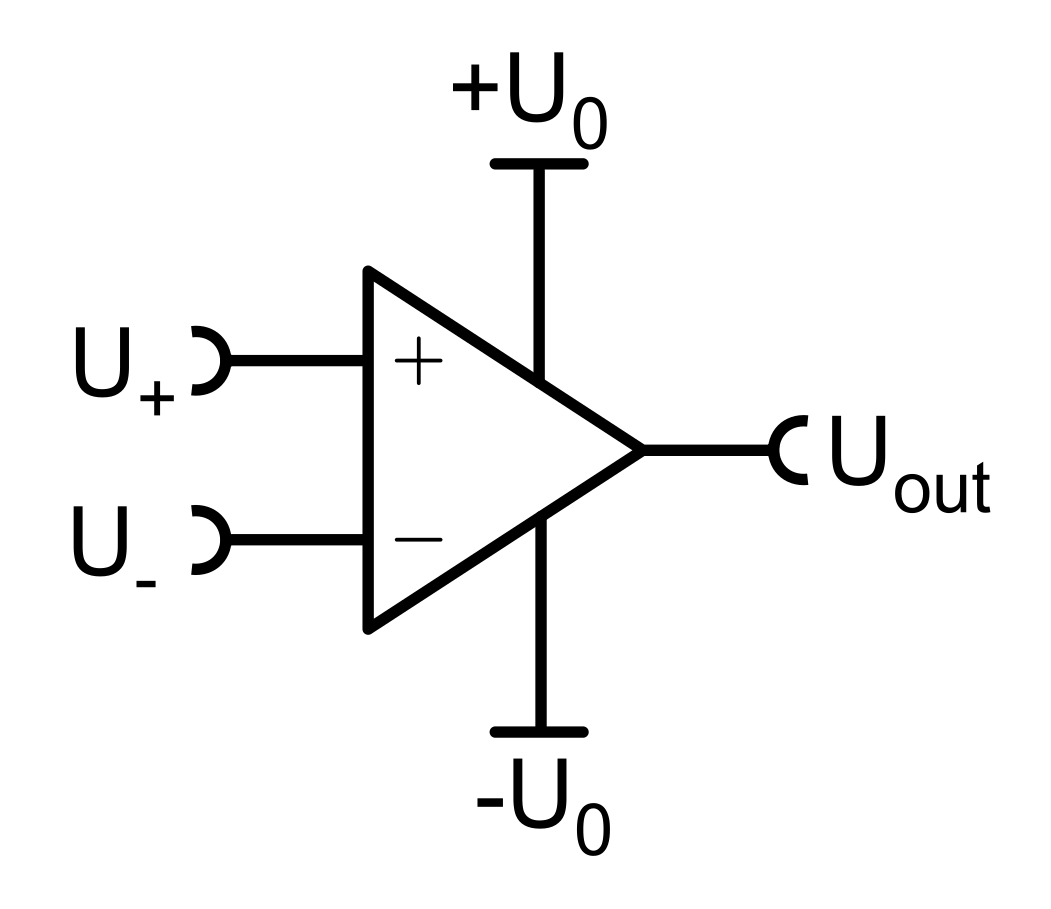
\includegraphics[width=0.5\textwidth]{opamp.png}
		\captionof{figure}{Schematic of an opamp; Abb.\ 5/6.1\cite{Praktikumsanleitung}}
	\end{Figure}
	\noindent The most important properties of opamps are
	\begin{enumerate}[label=--]
		\item With stable negative feedback, the opamp regulates the output voltage such that $U_+=U_-$.
		\item There is close to no input current $I_+=I_-\approx 0$.
	\end{enumerate}
	Important features of real opamps to keep in mind
	\begin{enumerate}[label=--]
		\item The maximum output voltage can't be higher than the maximum supply voltage.
		\item Due to internal constrains, the opamp has a finit slew rate, meaning that it can't change a signal at infinite speed.
		\item The open--loop gain decreases with rising frequency.
		      The bandwidth is the cutoff frequency at which $\nu =\tfrac{1}{\,\sqrt[]{2}}$.
		\item For $U_+=U_-=0$ one would assume that $U_\text{out}=0$.
		      In real world opamps this is not the case.
		      The output voltage goes to zero at a certain difference between $U_+$ and $U_-$.
		      This difference is component specific.
		\item The output voltage should not change if both input voltages increae at the same rate.
		      This is not the case in the real world.
		      The common mode rejection ratio is the ratio between the differential gain and common mode gain.
	\end{enumerate}
	The opamp can be utilised as a non--inverting amplifier with an ideal open--loop gain of infinity.
	Here $U_-=k\cdot U_\text{out}$ and $U_+=U_\text{in}$.
	The gain is
	\begin{align}
		\nu =\dfrac{U_\text{out}}{U_\text{in}}=\dfrac{1}{k}=1+\dfrac{Z_2}{Z_1}
		.\end{align}
	\begin{Figure}
		\centering
		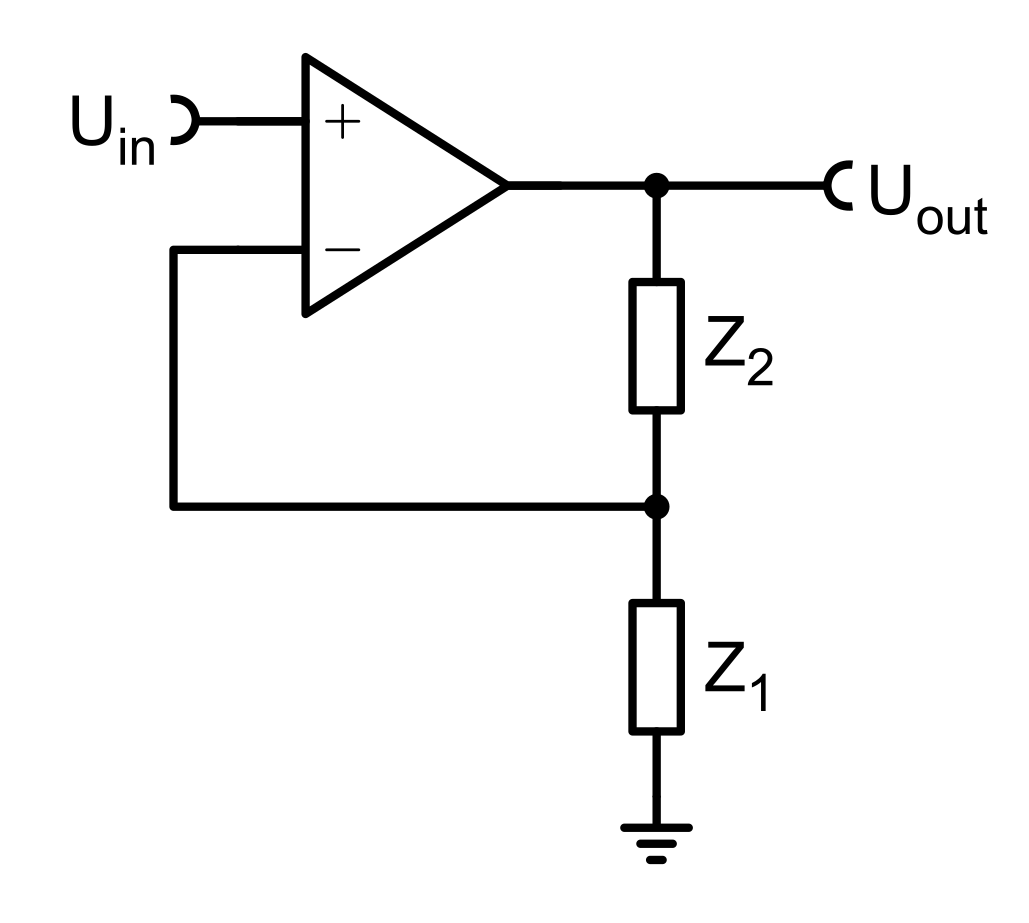
\includegraphics[width=0.6\textwidth]{noninverting_amp.png}
		\captionof{figure}{Non--inverting amplifier; Abb.\ 5/6.4\cite{Praktikumsanleitung}} \label{fig:non--inverting amplifier}
	\end{Figure}
	\noindent The opamp can also be used as an adder.
	As discussed in \hyperref[pre:F]{preliminary task F} the output voltage is an addition of input voltages
	\begin{align}
		U_\text{out}=c_iU_i\qquad c_i=-\dfrac{R_0}{R_i}
		.\end{align}
	\begin{Figure}
		\centering
		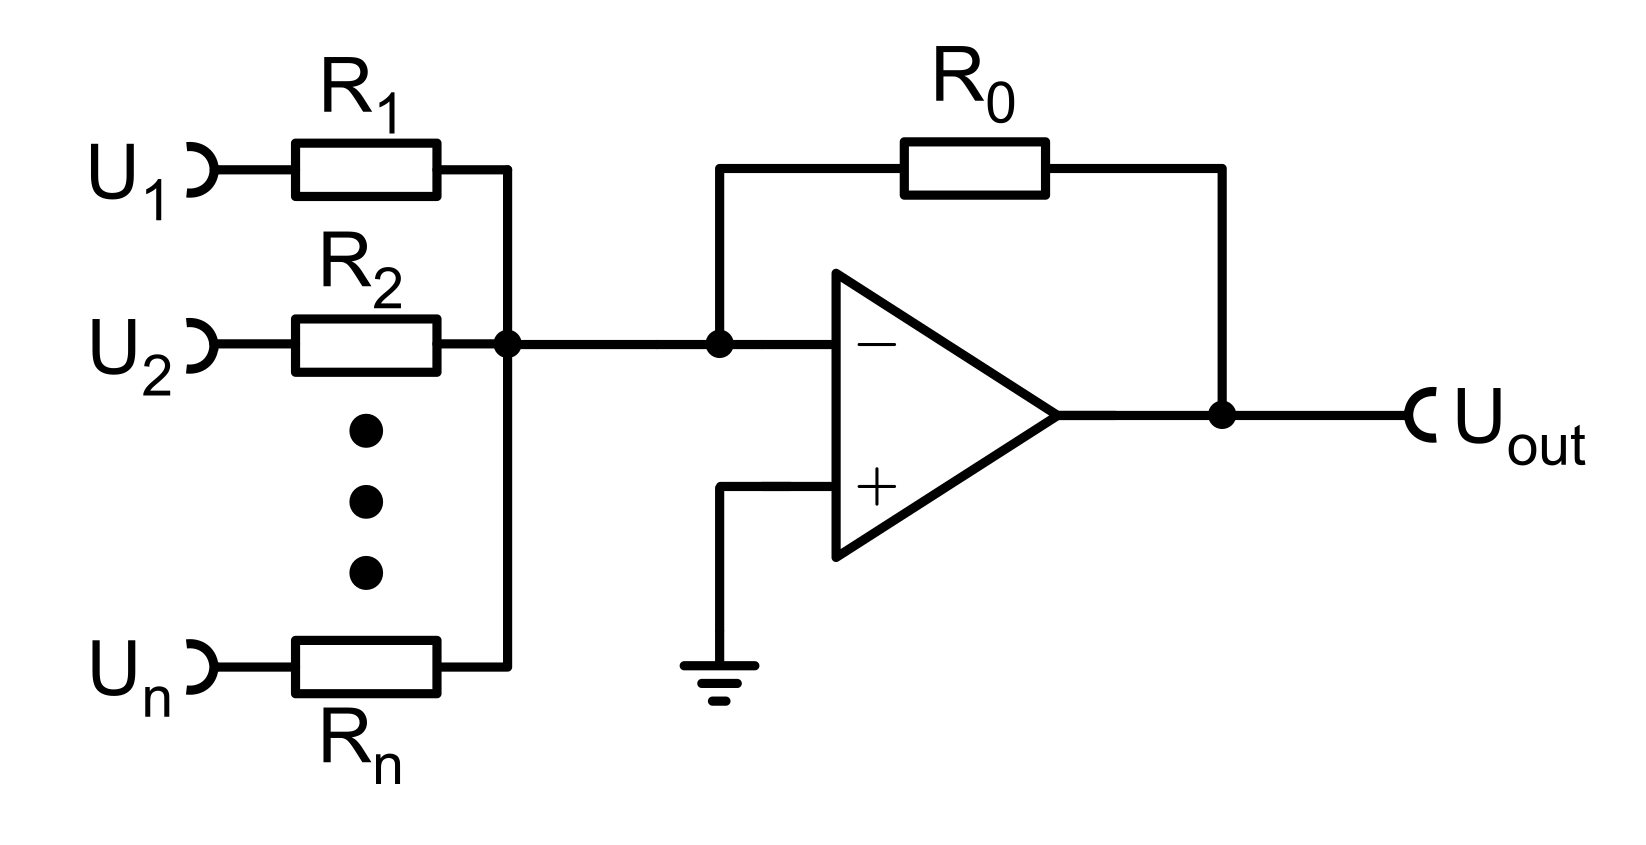
\includegraphics[width=0.6\textwidth]{adder.png}
		\captionof{figure}{Adder; Abb.\ 5/6.6\cite{Praktikumsanleitung}}
	\end{Figure}
	\noindent The opamp can also integrate signals by charging a capacitor to sum up the input signal
	\begin{align}
		U_\text{out}\left(t\right)=-\dfrac{1}{R_1C}\int_{t_0}^{t}U_\text{in}\left(t'\right)\td t'
		.\end{align}
	\begin{Figure}
		\centering
		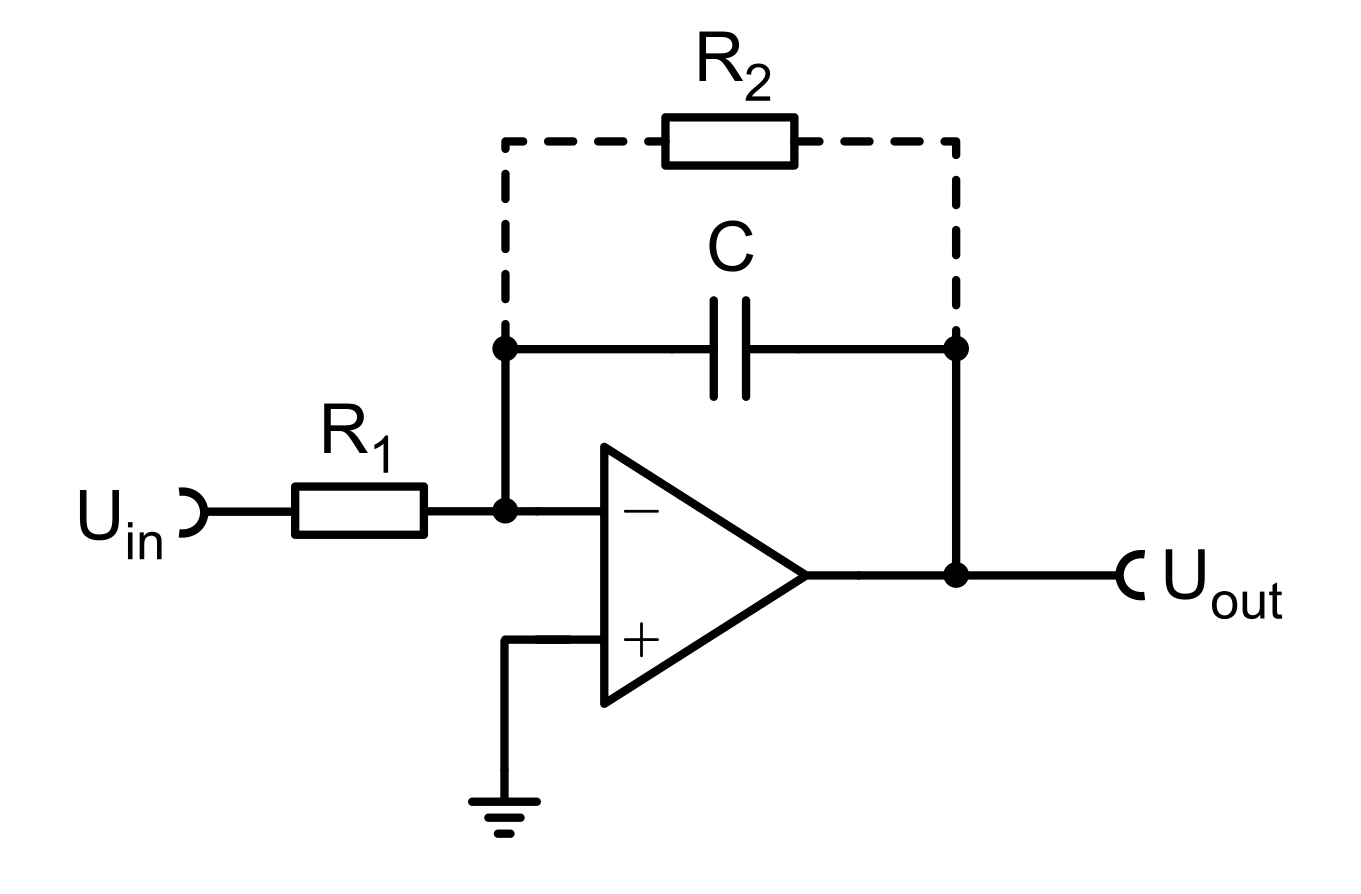
\includegraphics[width=0.6\textwidth]{integrator.png}
		\captionof{figure}{Integrator; Abb.\ 5/6.11\cite{Praktikumsanleitung}}
	\end{Figure}
	\noindent At last the opamp is used in a circuit to function as a differential amplifier.
	As discussed in \hyperref[pre:G]{preliminary task G}, the output voltage is an amplification of the difference of the input voltages
	\begin{align}
		U_\text{out}=\dfrac{R_2}{R_1}\left(U_2-U_1\right)
		.\end{align}
	Here $\tfrac{R_2}{R_1}$ is the gain.
	\begin{Figure}
		\centering
		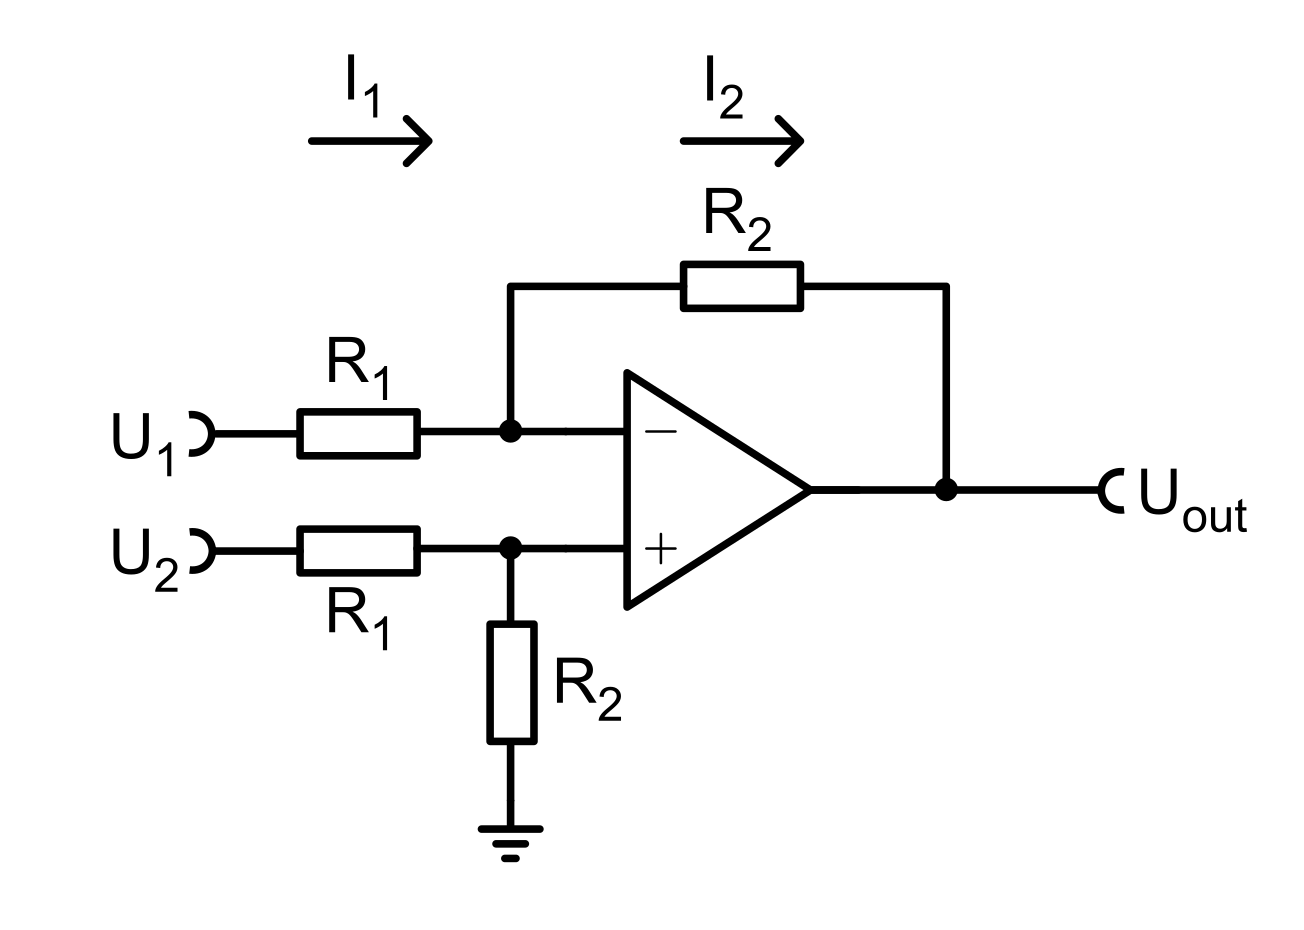
\includegraphics[width=0.6\textwidth]{differential_amp.png}
		\captionof{figure}{Differential amplifier; Abb.\ 5/6.7\cite{Praktikumsanleitung}}
	\end{Figure}
	\noindent When using the opamp as an inverting amplifier, the current flowing through the negative feedback circuit does not depend on $Z_2$ but only on $U_\text{in}$ and $Z_1$.
	Thus one can construct a current source for the resistance $Z_2$ which can be controlled via the input voltage.
	\begin{Figure}
		\centering
		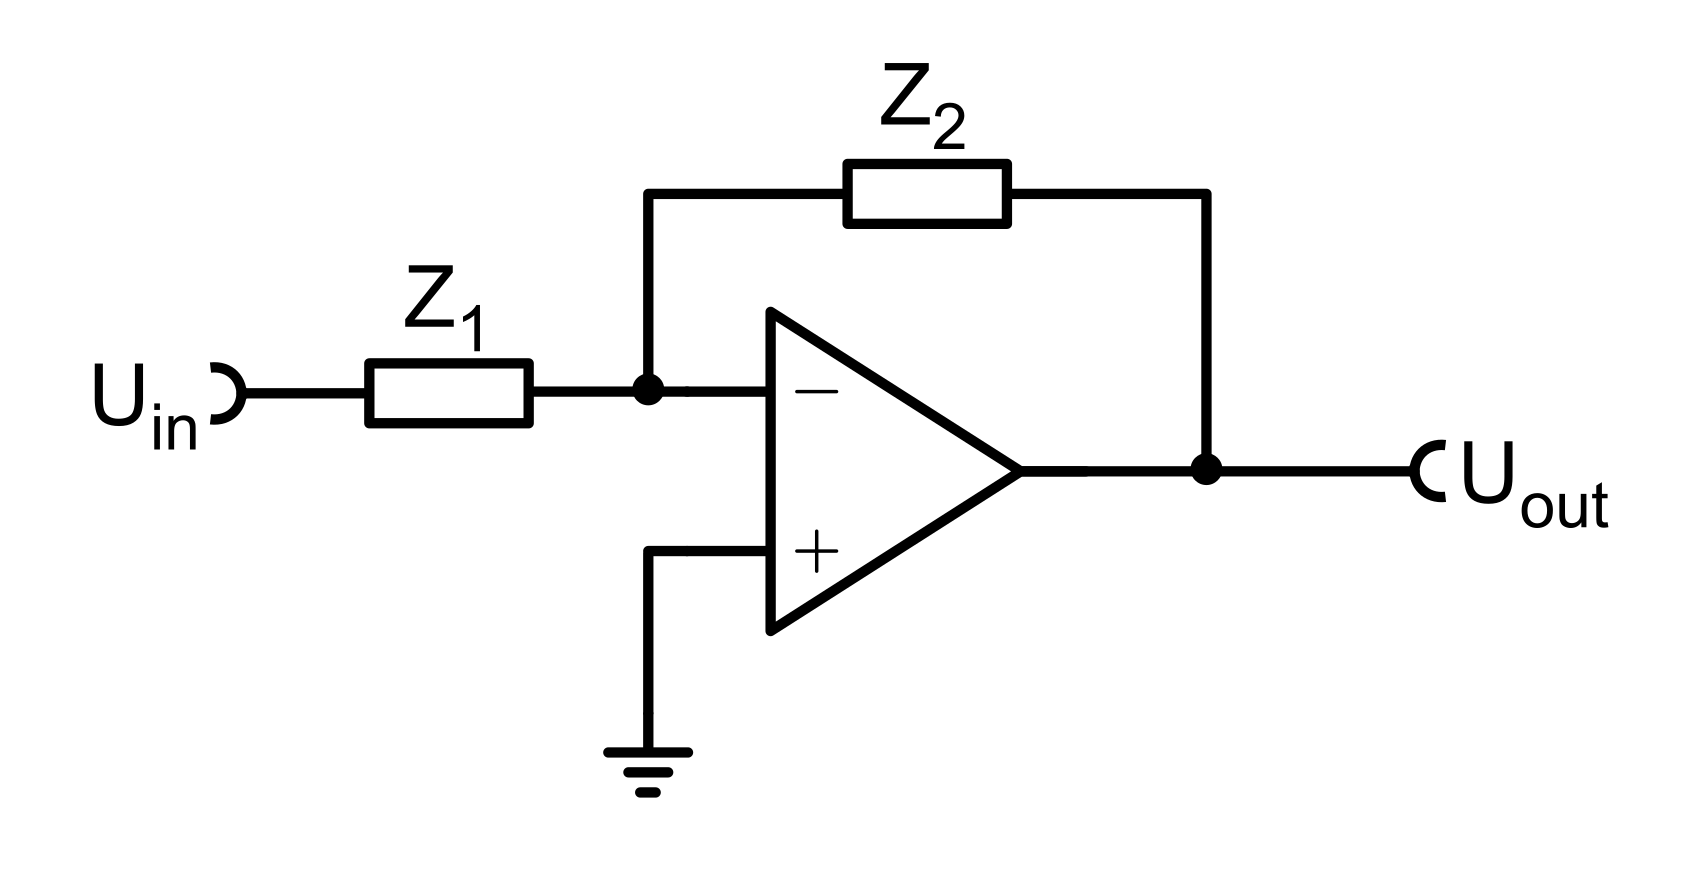
\includegraphics[width=0.6\textwidth]{inverting_amp.png}
		\captionof{figure}{Inverting amplifier; Abb.\ 5/6.5\cite{Praktikumsanleitung}}
	\end{Figure}
	\noindent The astable multivibrator uses the \textsc{Schmitt}--trigger to construct a signal from an ideal wave form, see \hyperref[pre:K]{preliminary task K}.
	\begin{Figure}
		\centering
		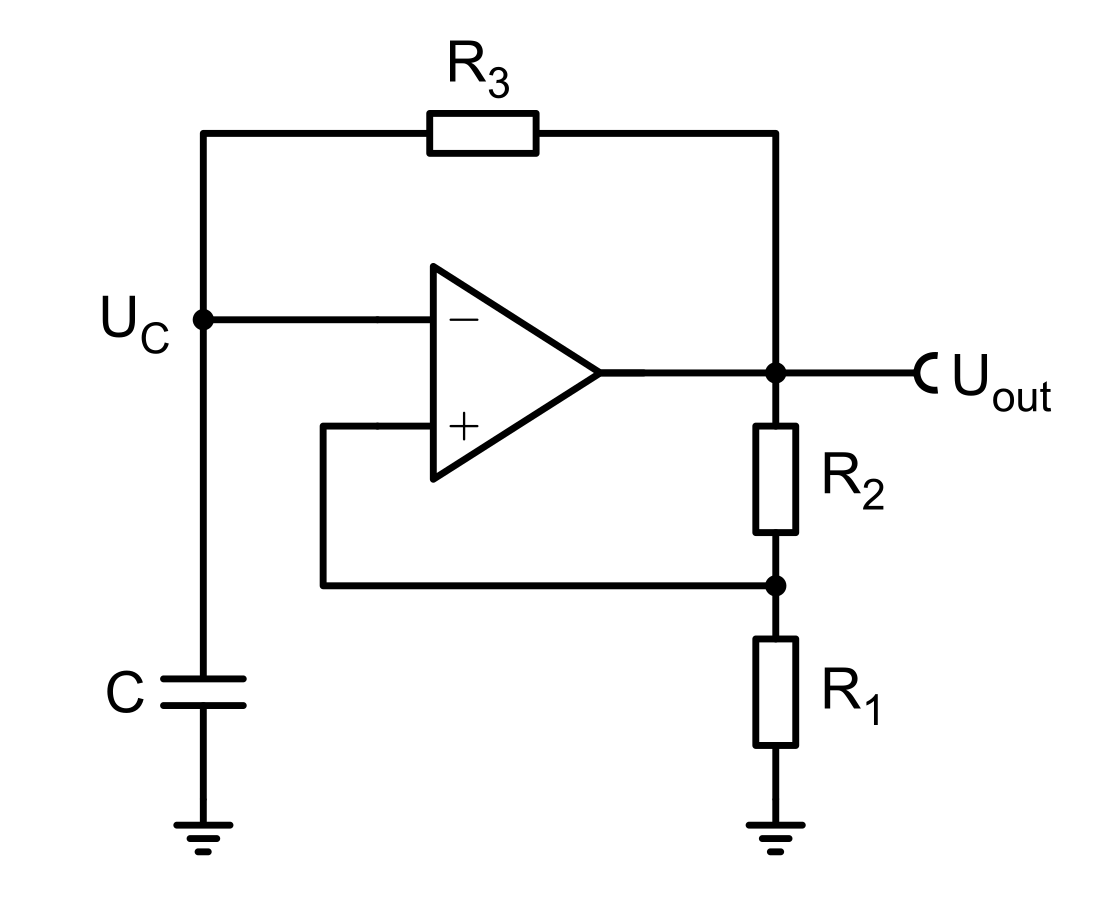
\includegraphics[width=0.6\textwidth]{astable_multivibrator.png}
		\captionof{figure}{Astable multivibrator; Abb.\ 5/6.15\cite{Praktikumsanleitung}}
	\end{Figure}

	\section{Preliminary Tasks}
	\subsection{A}
	The equation hold
	\begin{align}
		\dfrac{1}{\nu } & =\dfrac{1}{\nu _0}+k & \nu & =\dfrac{1}{\tfrac{1}{\nu _0}+k}
		.\end{align}
	For $k=0.1$, $\nu _0=10^4$ and $\nu _0=10^5$
	\begin{align}
		\nu _1 & \approx 9.990 & \nu _2 & \approx 9.999
		.\end{align}
	The approximation $\nu =\tfrac{1}{k}$ results in
	\begin{align}
		\nu _\text{Näh} & =10
		.\end{align}
	The deviation of $\nu _1$ and $\nu _2$ from $\nu _\text{Näh}$ lie at $0.001\%$ and $0.0001\%$ respectively.

	\subsection{B}
	It hold
	\begin{align}
		 &  &                 &  & U_x & = U_\text{in}-kU_\text{out}    &  &  &  &           \\
		 &  & \Leftrightarrow &  &     & = U_\text{in}-kv_0U_x          &  &  &  & \nonumber \\
		 &  & \Leftrightarrow &  &     & = \dfrac{U_\text{in}}{1+v_0k}. &  &  &  &
	\end{align}
	For $k=0.1$, $v_0=10^5$ and $U_\text{in}=\SI{1}{V}$
	\begin{align}
		U_x\approx \SI{0.0001}{V}
		.\end{align}

	\subsection{C}
	Let there be a common mode signal with $\Delta U_+=\Delta U_-=+\Delta U_\text{in}$.
	then
	\begin{align}
		 &  &  &  & \Delta U_+ & = \Delta U_E+\Delta U_1 & \Delta U_- & = \Delta U_E+\Delta U_1. &  &  &  &
	\end{align}
	from this follows $\Delta U_\text{in}=\Delta U_E+\Delta U_1$.
	The output voltage is
	\begin{align}
		\Delta U_\text{out}=R_C\cdot \Delta I_C
		.\end{align}
	At point 1,
	\begin{align}
		I_1=2I_E
		.\end{align}
	Therefore
	\begin{multline}
		\Delta U_\text{in} = R_E\cdot \Delta I_E+R_1 \cdot 2\Delta I_E \\= \Delta I_E\left(R_E+2R_1\right)\approx \Delta I_E\cdot 2R_1.
	\end{multline}
	At the node $U_\text{out}$ applies
	\begin{align}
		\Delta I_E=\Delta I_C\Rightarrow \Delta U_\text{out}=R_C\cdot \Delta I_E
		.\end{align}
	The amplification results in
	\begin{align}
		v_{CM}=\dfrac{\Delta U_\text{out}}{\Delta U_\text{in}}=\dfrac{R_C}{2R_1}
		.\end{align}
	The common mode suppression is
	\begin{align}
		10\log \left(\dfrac{R_E}{R_1}\right)=10\log \left(\dfrac{\SI{1}{\kilo\ohm}}{\SI{100}{\kilo\ohm}}\right)=-\SI{20}{dB}
		.\end{align}

	\subsection{D}
	The frequency dependence of the impedance of a capacitor is
	\begin{align}
		Z_1   & = \dfrac{1}{\text{i}\omega C}=\dfrac{1}{\text{i}2\pi fC}        \\
		|Z_1| & = \left|\dfrac{1}{\text{i}\omega C}\right| = \dfrac{1}{2\pi fC}
		.\end{align}
	The gain as a function of frequency is
	\begin{align}
		v\left(f\right)=1+\dfrac{Z_2}{|Z_1|}=1+R2\pi fC
		.\end{align}
	The limits are
	\begin{align}
		\lim_{f \rightarrow 0}\left[1+R2\pi fC\right] & = 1 & \lim_{f \rightarrow \infty}\left[1+R2\pi fC\right] & = \infty
		.\end{align}
	For $|Z_1| = R$ it has to hold that
	\begin{align}
		\dfrac{1}{2\pi fC}=R\Leftrightarrow f=\dfrac{1}{2\pi RC}
		.\end{align}
	With concrete values $Z_1=R=\SI{100}{\kilo\ohm}$ and $Z_1=C=\SI{100}{\nano F}$, the frequency is
	\begin{align}
		f=\dfrac{1}{2\pi RC}\approx \SI{15.92}{Hz}\Rightarrow v\left(f\right)\approx 2
		.\end{align}
	\begin{Figure}
		\centering
		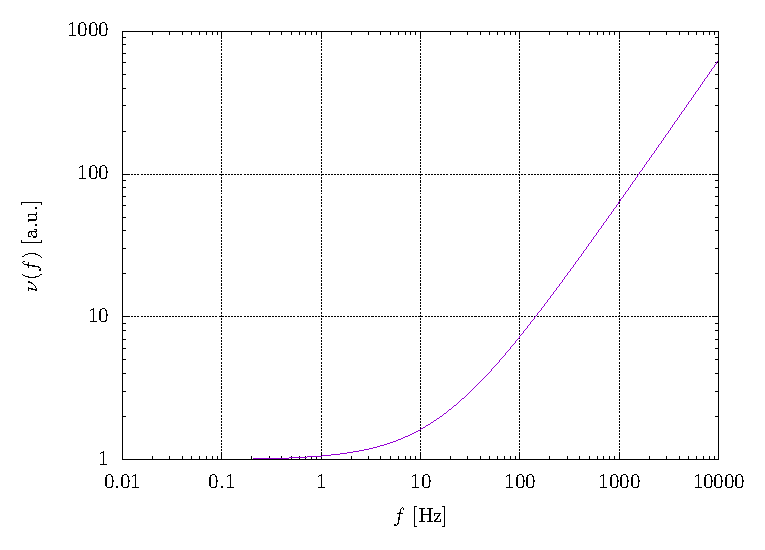
\includegraphics[width=0.7\textwidth]{../plot/preE_crop.pdf}
		\captionof{figure}{Time dependend amplification of a non--invertible amplifier as a \textsc{Bode}--plot}
	\end{Figure}

	\subsection{E}
	Let
	\begin{align}
		v=\dfrac{U_\text{out}}{U_\text{in}}=-\dfrac{Z_2}{Z_1}
		.\end{align}
	The minus sign results from the negative feedback.
	Because of the golden rule $U_-=U_+=\SI{0}{V}$, the negative feedback has a different sign compared to the input signal.
	\\\indent The input impedance is very high and the output impedance very low.

	\subsection{F} \label{pre:F}
	The first \textsc{Kirchhoff}'s law states (\textsc{Einstein} notation)
	\begin{align}
		                &  &  &  & \sum_{i}^{}I_i       & = -I_\text{out}              &  &  &  & \\
		\Leftrightarrow &  &  &  & \dfrac{U_i}{R_i}     & = -\dfrac{U_\text{out}}{R_0} &  &  &  & \\
		\Leftrightarrow &  &  &  & -\dfrac{R_0}{R_i}U_i & = U_\text{out}               &  &  &  & \\
		\Leftrightarrow &  &  &  & c_iU_i               & = U_\text{out}.              &  &  &  &
	\end{align}

	\subsection{G} \label{pre:G}
	\begin{align}
		 &  &  &  & U_+ & = U_2\dfrac{R_2}{R_1+R_2}      &  &  &  & |\text{voltage divider}    \\
		 &  &  &  & U_- & = U_+                          &  &  &  & |\text{golden rule}        \\
		 &  &  &  & I_1 & = \dfrac{U_1-U_-}{R_1}         &  &  &  & |\text{\textsc{Ohm}'s law} \\
		 &  &  &  & I_2 & = I_1                          &  &  &  & |\text{golden rule}        \\
		 &  &  &  & I_2 & = \dfrac{U_-U_\text{out}}{R_2} &  &  &  & |\text{\textsc{Ohm}'s law}
		.\end{align}
	The final result $U_\text{out}=\tfrac{R_2}{R_1}\left(U_2-U_1\right)$ can be calculated using the above relations.

	\subsection{H}
	A constant negative input voltage provides a continuous charge to the capacitor, resulting in a steadily rising output voltage.
	One could also argue that for a constant input voltage the integral will increase linearly.

	\subsection{I}
	For an inverting amplifier $\nu =-\tfrac{Z_2}{Z_1}$.
	With $Z_1=R$ and $Z_2=\tfrac{1}{\text{i}\omega C}$
	\begin{align}
		 &  &  &  & \nu & = -\dfrac{1}{\text{i}\omega CR}. &  &  &  &
	\end{align}
	The phase relation between the output-- and inputsignal is then
	\begin{align}
		\tan \Phi & = \dfrac{\mathfrak{I}\left(\nu \right)}{\mathfrak{R}\left(\nu \right)}=\lim_{\alpha \rightarrow 0}\dfrac{-\tfrac{1}{\omega CR}}{\alpha }=-\infty
		.\end{align}
	Thus $\Phi =-\tfrac{\pi }{2}$.

	\subsection{J}
	The AD711 opamp has a slew rate of $s=\SI{20}{V.\micro s ^{-1}}$.
	The peak to peak voltage lies at $U_{p p}=\SI{28}{V}$.
	This means that the AD711 needs
	\begin{align}
		t=\dfrac{U_{p p}}{s}=\SI{1.4}{\micro s}
	\end{align}
	to get from $\SI{-14}{V}$ to $\SI{+14}{V}$.
	The switching frequency is therefore
	\begin{align}
		\tfrac{1}{t}=\SI{0.714}{\micro s ^{-1}}
		.\end{align}

	\subsection{K} \label{pre:K}
	\begin{Figure}
		\centering
		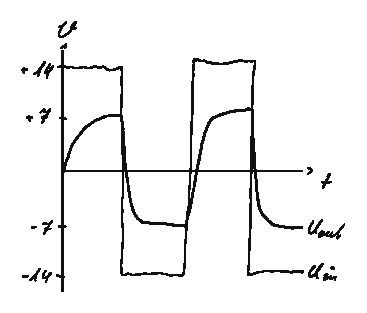
\includegraphics[width=\textwidth]{../plot/preK_crop.pdf}
		\captionof{figure}{Astable multivibrator, voltage curve}
	\end{Figure}
	\noindent The ideal signal is a square--wave with $U_\text{max,min}\pm \SI{14}{V}$.
	Due to the slew rate of the opamp, the signal need time to rise to $\pm \si{7}{V}$.
	The output voltage can be modeled with an exponential function.

	\newpage
	\section{Analysis}
        \subsection{Non--inverting amplifier}
        The \hyperref[fig:non--inverting amplifier]{non--inverting amplifier} is built with a gain of $\nu =11$ (i.e.\ $R_1=\SI{1}{k\ohm}$ and $R_2=\SI{10}{k\ohm}$).
        A signal of $U_{p p}=\SI{1}{V}$ is applied to the circuit and the gain is observed for different frequencies.
        \begin{Figure}
                \centering
                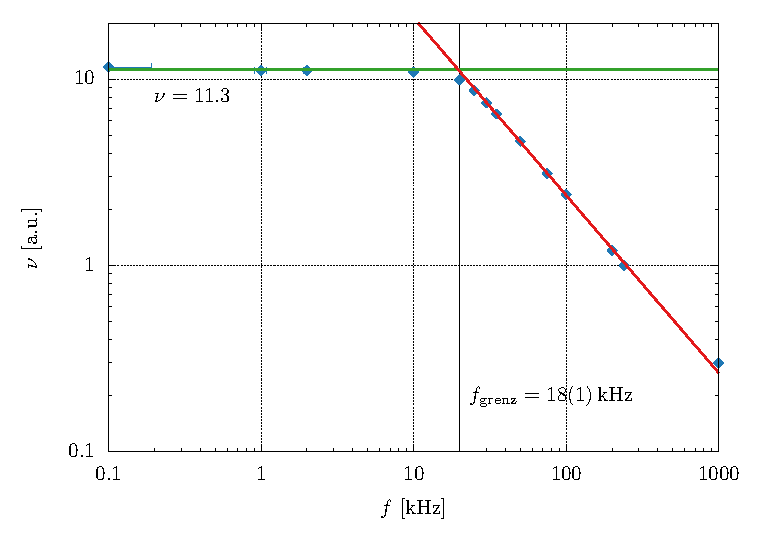
\includegraphics[width=0.6\textwidth]{../plot/5_1_2_crop.pdf}
                \captionof{figure}{\textsc{Bode}--plot of a non--inverting amplifier with $\nu =11$} \label{fig:bode-plot}
        \end{Figure}
        \noindent As one can see, up to $f_\text{grenz}\approx \SI{18+-1}{kHz}$ the gain stays the same (at $\nu \approx 11.3$).
        After $f_\text{grenz}$ the gain decreases exponentially and is 1 at $f_T=\SI{240}{kHz}$.
        \begin{center}
                \begin{tabular}{|c|c|}
                        \hline
                        frequency $f$ [kHz] & gain $\nu $ [a.u.]\\
                        \hline
                        0.30 & 1000\\
                        1.00 & 240\\
                        1.20 & 200\\
                        2.40 & 100\\
                        3.12 & 75\\
                        4.65 & 50\\
                        6.50 & 35\\
                        7.48 & 30\\
                        8.69 & 25\\
                        9.92 & 20\\
                        10.9 & 10\\
                        11.1 & 2\\
                        11.1 & 1\\
                        11.6 & 0.1\\
                        11.5 & 0.01\\
                        \hline
                \end{tabular}
                \captionof{table}{Values for \hyperref[fig:bode-plot]{\textsc{Bode}--plot}}
        \end{center}
        \noindent
        Because the opamp model LM301AP is not listed in the protocoll and has no onilne documentation it is not possible to compare the measured transit frequency to the exact value.
        \\\\\noindent Now the gain is set to $\nu =101$ by using $R_2=\SI{470}{k\ohm}$ and $R_1=\SI{4.7}{k\ohm}$.
        The signal has a peak to peak voltage of $\SI{100}{mV}$.
        \begin{Figure}
                \centering
                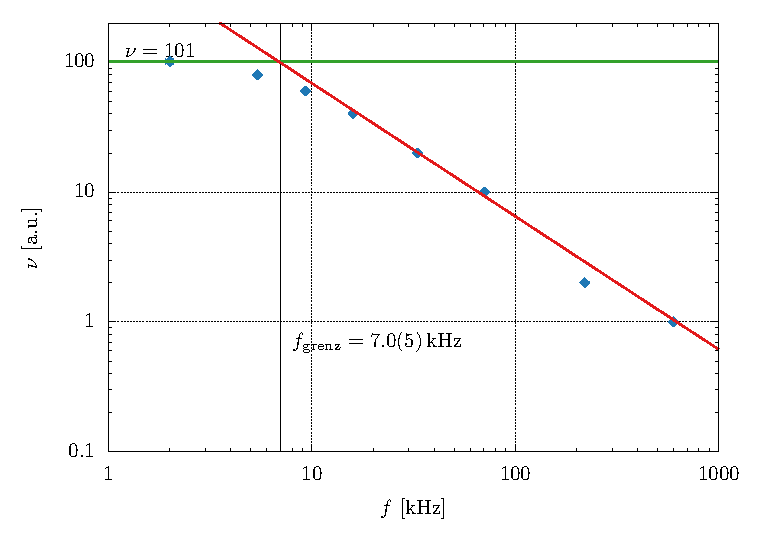
\includegraphics[width=0.6\textwidth]{../plot/5_1_2_2_crop.pdf}
                \captionof{figure}{\textsc{Bode}--plot for different gain}
        \end{Figure}
        The cutoff frequency lies at $f_\text{grenz}=\SI{7+-0.5}{kHz}$; the transit frequency lies at $f_T=\SI{600}{kHz}$.
        For $\nu =2$ the frequency lies at $f_2=\SI{220}{kHz}$.
        Due to the heavy negative feedback, the amplification decreases linear (in the loglog plot).
        \\\\ For $\nu =101$ a square--wave signal with frequency of $f=\SI{1}{kHz}$ and $U_{p p}=\SI{20}{V}$ is set.
        \begin{Figure}
                \centering
                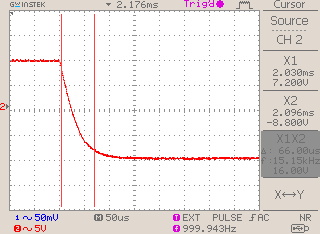
\includegraphics[width=0.6\textwidth]{../data/DS0026_negate.png}
                \captionof{figure}{Slew rate for said square--wave}
        \end{Figure}
        \noindent The slew rate is the time it takes the oscillograph to raise a signal from 10\% to 90\%.
        From the cursors on the oszillogramm, one can see the time difference to be $\Delta =\SI{66}{\micro s}$.
        \\\indent When increasing the frequency, the slew rate stays the same, because the slew rate is an intrinsic property of the oscillograph and should not change if any outside parameters change.
        The amplitude decreases as the frequency increases because the plateaus of constant voltage shorten.
        If the frequency is high enough, the signal will change polarity too fast for the circuit to be complete saturated.
        There are no differences to the sine signal.
        The slew rate is also not relevant for the sine signal, because it does not switch sign instantly.
        \\\\ Now a gain of $\nu =11$ (with $R_1=\SI{10}{k\ohm}$ and $R_2=\SI{100}{k\ohm}$) is set and a capacitor with $C=\SI{0.1}{\micro F}$ is connected in series with $R_1$.
        Due to different unkown reasons, like a loose connection in a cable, nothing seemed to have changend, when connecting the capacitor.
        Our expectation was that the capacitor and resistor would behave like a high--pass, meaning that signals with high frequencies would rather run through the capacitor into ground than the opamp, resulting in high frequency signals not being amplified.

	\subsection{Adder}
	With the help of Tri-Sinewave-Generator we generate three Sinewaves with \SI{50}{Hz}, \SI{100}{Hz} and \SI{150}{Hz}. The goal is to produce a sawtooth-signal. For that we look at the taylor expansion and find the amplitudes for our frequencies.
	\begin{align}
		F(t)=\frac{2}{\pi}A\cdot\left(\sin{\omega t}+\frac{1}{2}\sin{2\omega t}+\frac{1}{3}\sin{3\omega t}+\dots\right)
	\end{align}
	So we choose for our \SI{50}{Hz} Signal full amplitude, for \SI{100}{Hz} halve amplitude and for \SI{150}{Hz} one third amplitude. With this configuration we achieve a signal thats displayed in fig. \ref{fig:calcsaw}.
	\begin{Figure}
		\centering
		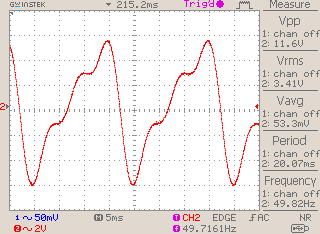
\includegraphics[width=1\textwidth]{../data/DS0031_n.png}
		\captionof{figure}{Sawtooth-Signal with calculated amplitudes}
		\label{fig:calcsaw}
	\end{Figure}
	We see that it allready approximates a Sawtooth-Signal pretty well. But we think we can make it even better. So we adjust our amplitudes and find an even better approximation. It is displayed in fig. \ref{fig:foundsaw}.
	\begin{Figure}
		\centering
		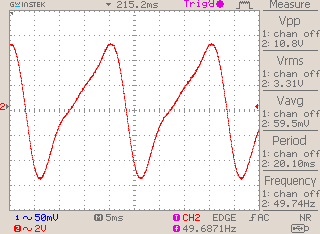
\includegraphics[width=1\textwidth]{../data/DS0030_n.png}
		\captionof{figure}{Sawtooth-Signal with found amplitudes}
		\label{fig:foundsaw}
	\end{Figure}
	For this Outputsignal we used
	\begin{align*}
		U(f=\SI{50}{Hz})  & =1\cdot U_0\text{,}               \\
		U(f=\SI{100}{Hz}) & =\frac{1}{2}\cdot U_0\text{\;and} \\
		U(f=\SI{150}{Hz}) & =\frac{1}{6}\cdot U_0\text{.}
	\end{align*}
	This difference from calculated to experimental optimum, could be a result of frequency dependent volatge, voltage loss from overlooked resistance or simply bad equipment.
	\subsection{Constant current source}
	In this subsection we build a constant current source circut, thats shown in the schematic in fig. \ref{fig:ccs}. We expect a current of $I_{R_2}=\frac{U}{R_1}=\frac{\SI{9.4}{V}}{\SI{47}{k\Omega}}=\SI{0.2}{mA}$. For $R_2$ we choose \SI{10}{k\Omega}.
	\begin{Figure}
		\centering
		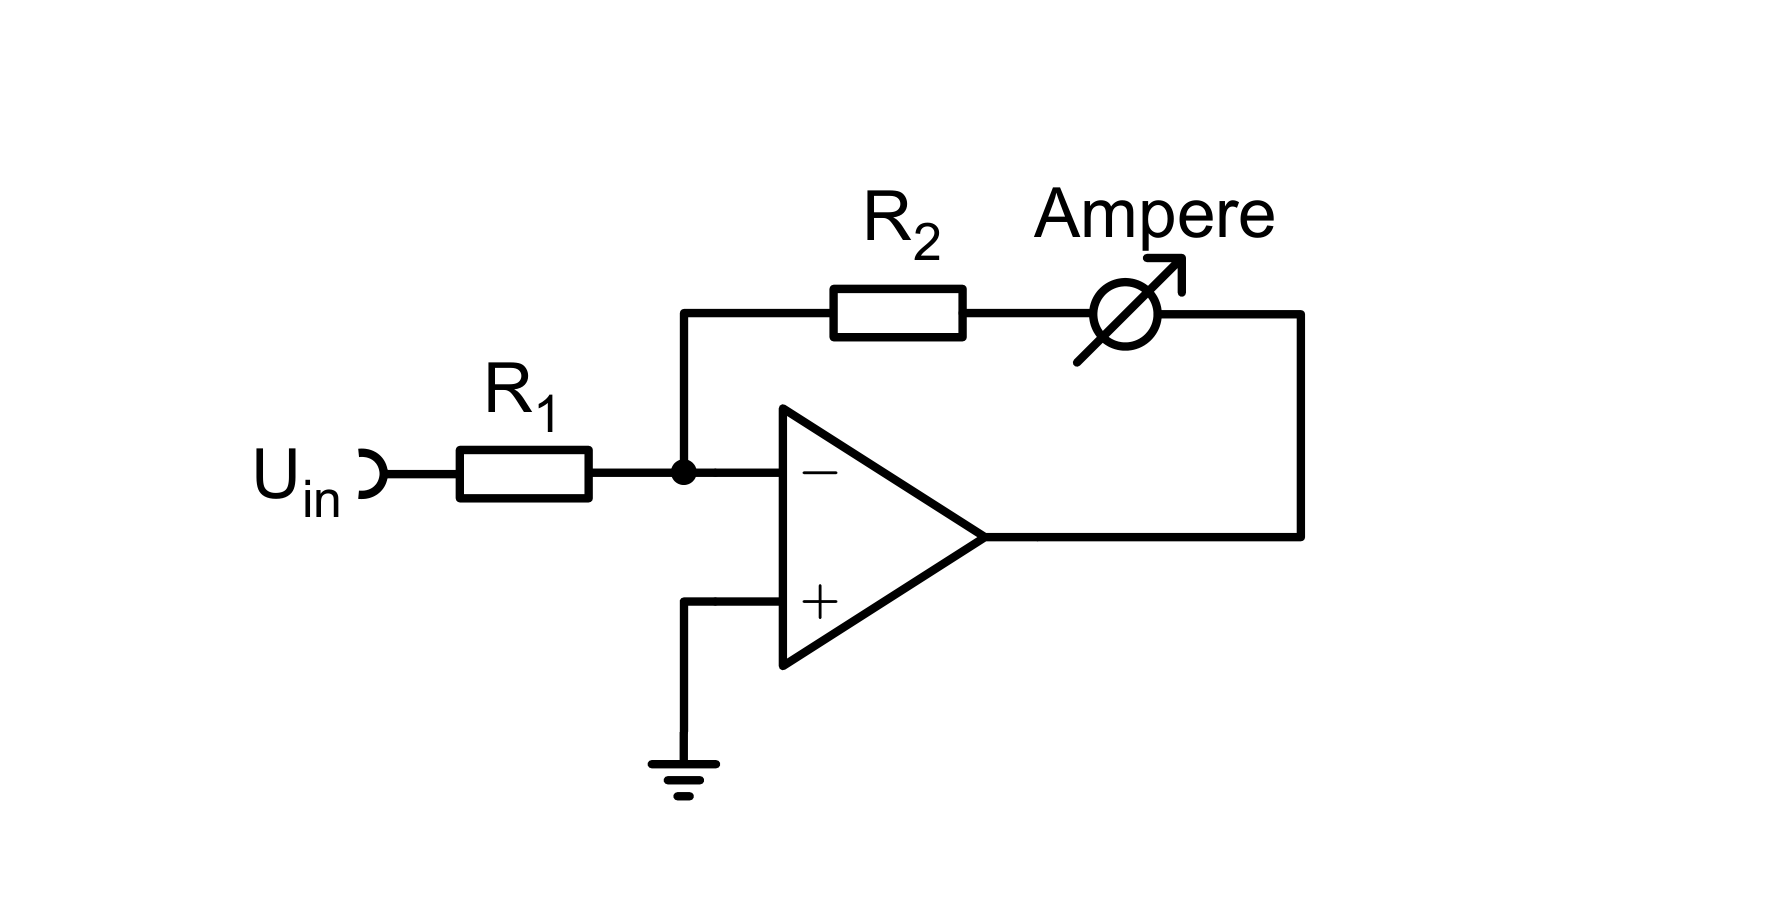
\includegraphics[width=1\textwidth]{conscurrentshematic.png}
		\captionof{figure}{Schematic of a constant current source \cite{Praktikumsanleitung}}
		\label{fig:ccs}
	\end{Figure}
	Before resistor 2 we meassure a current of \SI{0.171}{\milli A}. Thats diviation of \SI{16.96}{\%} from the calculated current. Causes could be again and as always resitance that we have overlooked or bad equipment. Especially with souch low current (micro to milli ampere), we can expect some diviations alone from the resistance in the cables and bad connections.

	Afterwards we replace the second resistor with a potentiometer and variate the resistance. We meassure no difference in the current. Thats as expected, since the feedback loop is supposed to do exactly that; regulate itself, since the output voltage will grow proportional to the input voltage, wich is less regulated by the higher resistor. With this idea we see that the outputvoltage will change with the change of the potentiometer. So we have to ways of reducing the current. Either we increase the first resistor or we reduce the input voltage.

	\subsection{Integrator}
	Now we substitute the second resistor / potentiometer and amperemeter with an \SI{1}{\mega \Omega} resistor and place a \SI{100}{\micro F} condesator parallel to it. We also set a square wave signal with \SI{100}{Hz} and \SI{1}{V_{PP}}. The resulting oscillogramm is displayed in fig. \ref{fig:int1} with CH1 beeing the input signal and CH2 the output signal.
	\begin{Figure}
		\centering
		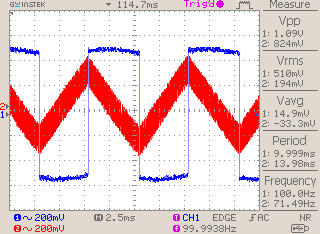
\includegraphics[width=1\textwidth]{../data/DS0032_n.png}
		\captionof{figure}{Integrator with a square wave signal with \SI{100}{Hz} and \SI{1}{V_{PP}}.}
		\label{fig:int1}
	\end{Figure}
	As expected the result is the integration of the input signal.

	Now we change the frequency. The result is displayed in fig. \ref{fig:int2} and \ref{fig:int3}.
	\begin{Figure}
		\centering
		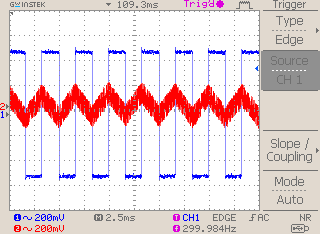
\includegraphics[width=1\textwidth]{../data/DS0033_n.png}
		\captionof{figure}{Integrator with a square wave signal with \SI{300}{Hz} and \SI{1}{V_{PP}}.}
		\label{fig:int2}
	\end{Figure}
	\begin{Figure}
		\centering
		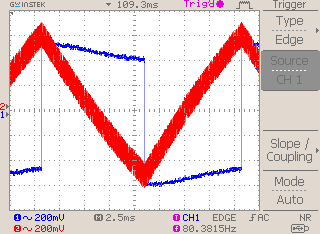
\includegraphics[width=1\textwidth]{../data/DS0034_n.png}
		\captionof{figure}{Integrator with a square wave signal with \SI{80}{Hz} and \SI{1}{V_{PP}}.}
		\label{fig:int3}
	\end{Figure}
	We observe that with higher frequencies, the integrated signal looses peak-to-peak voltage. Thats logical since, firstly the condensator increases resistence with higher frequencies, and secondly if we think about it in a mathmatical sense, integrating a square wave signal with shorter pulses, gives the integration less time to increase, so the voltage does not increase as much.

	Now we change input voltage. The result is displayed in fig. \ref{fig:int4}, \ref{fig:int5} and \ref{fig:int6}.
	\begin{Figure}
		\centering
		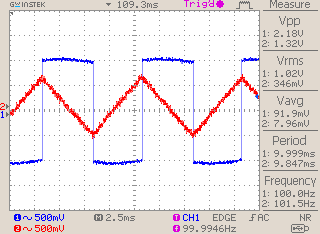
\includegraphics[width=1\textwidth]{../data/DS0035_n.png}
		\captionof{figure}{Integrator with a square wave signal with \SI{100}{Hz} and \SI{2}{V_{PP}}.}
		\label{fig:int4}
	\end{Figure}
	\begin{Figure}
		\centering
		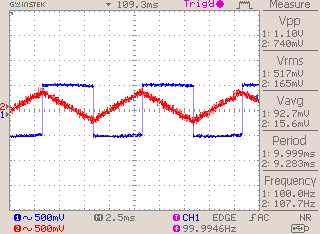
\includegraphics[width=1\textwidth]{../data/DS0036_n.png}
		\captionof{figure}{Integrator with a square wave signal with \SI{100}{Hz} and \SI{1}{V_{PP}}.}
		\label{fig:int5}
	\end{Figure}
	\begin{Figure}
		\centering
		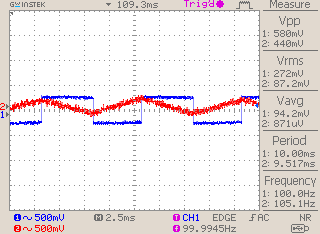
\includegraphics[width=1\textwidth]{../data/DS0037_n.png}
		\captionof{figure}{Integrator with a square wave signal with \SI{100}{Hz} and \SI{0.5}{V_{PP}}.}
		\label{fig:int6}
	\end{Figure}
	As we see, the input and output voltages are proportionaly lowerd as we descend from \SI{2}{V_{PP}} to \SI{0.5}{V_{PP}}. Thats not so surprising since every component scales the voltage linealy through its resistance.

	If we remove the \SI{1}{\mega \Omega} resistor we can occasionlly observe fracmentations, wich are displayed in fig. \ref{fig:int7}.
	\begin{Figure}
		\centering
		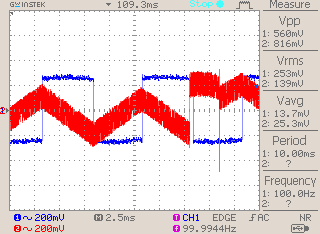
\includegraphics[width=1\textwidth]{../data/DS0038_n.png}
		\captionof{figure}{Integrator wihtout \SI{1}{\mega\Omega} resistor with a square wave signal with \SI{100}{Hz} and \SI{0.5}{V_{PP}}.}
		\label{fig:int7}
	\end{Figure}
	We suspect that the base-line voltage is the cause of the phenomenon, since there is no resistance over wich it can decrease and every fluctuation, noise and base-voltage is captured by the capacitor/integrator.

	Switching the input signal to a sine wave, gives us the expected cosine wave displayd in fig. \ref{fig:int8}. The drop in voltage is explainable through overlooked resistances or frequency dependent resistance.
	\begin{Figure}
		\centering
		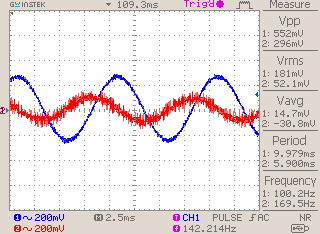
\includegraphics[width=1\textwidth]{../data/DS0041_n.png}
		\captionof{figure}{Integration of a sine wave.}
		\label{fig:int8}
	\end{Figure}
	Displaying the phases through XY configuration we can observe the Lissajour figure in fig. \ref{fig:int9}
	\begin{Figure}
		\centering
		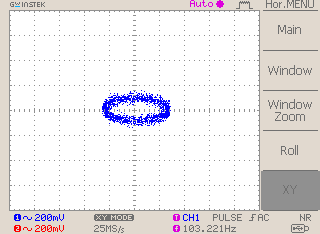
\includegraphics[width=1\textwidth]{../data/DS0040_n.png}
		\captionof{figure}{Lissajour figure of the sine wave and its integrated cosine output.}
		\label{fig:int9}
	\end{Figure}

	Now we increase the voltage and observe a proportional increase in the output signal (fig. \ref{fig:int10}), where as the ellips (fig. \ref{fig:int11}) just increases in size in x and y direction.
	\begin{Figure}
		\centering
		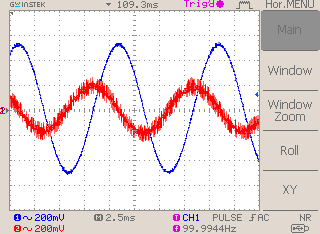
\includegraphics[width=1\textwidth]{../data/DS0043_n.png}
		\captionof{figure}{Integration of a sine wave with \SI{100}{Hz} and \SI{1}{V_{PP} }}
		\label{fig:int10}
	\end{Figure}
	\begin{Figure}
		\centering
		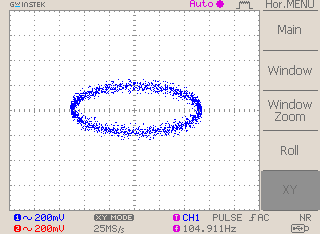
\includegraphics[width=1\textwidth]{../data/DS0042_n.png}
		\captionof{figure}{Integration of a sine wave with \SI{100}{Hz} and \SI{1}{V_{PP}} in XY channel configuration as Lissajour figure.}
		\label{fig:int11}
	\end{Figure}

	Now we can also decrease the frequency from \SI{100}{Hz} to \SI{40}{Hz}. We observe that the ouput signal is increased to nearly the level of the input signal. This behaviour suggests that indeed the voltage is frequeny dependent, wich makes sense, since the impedance of the capacitor is also frequency dependent. We also observe a nearly perfect circel instead of a ellipse.
	\begin{Figure}
		\centering
		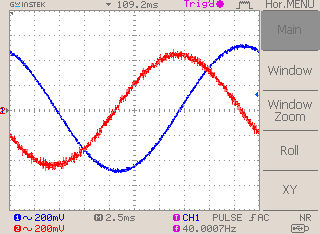
\includegraphics[width=1\textwidth]{../data/DS0045_n.png}
		\captionof{figure}{Integration of a sine wave with \SI{40}{Hz} and \SI{1}{V_{PP} }}
		\label{fig:int12}
	\end{Figure}
	\begin{Figure}
		\centering
		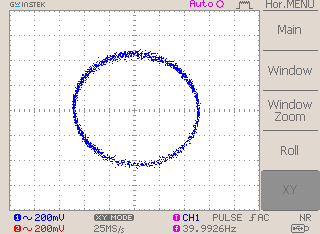
\includegraphics[width=1\textwidth]{../data/DS0044_n.png}
		\captionof{figure}{Integration of a sine wave with \SI{40}{Hz} and \SI{1}{V_{PP}} in XY channel configuration as Lissajour figure.}
		\label{fig:int13}
	\end{Figure}

	\subsection{Differential amplifier}
	At last we look back again at the differential amplifier and analyse the effect of applying a positiv base voltage at the the positiv input, wich is parallel connected to ground. As we can see in fig. \ref{fig:damp1}, \ref{fig:damp2} and \ref{fig:damp3}, that the increasing base line voltage increases the shift in its output.
	\begin{Figure}
		\centering
		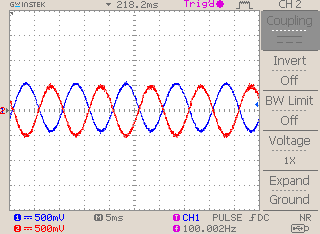
\includegraphics[width=1\textwidth]{../data/DS0047_n.png}
		\captionof{figure}{Amplification of a sine wave with no base voltage.}
		\label{fig:damp1}
	\end{Figure}
	\begin{Figure}
		\centering
		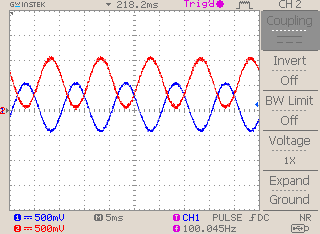
\includegraphics[width=1\textwidth]{../data/DS0048_n.png}
		\captionof{figure}{Amplification of a sine wave with a base voltage of \SI{0.5}{V}.}
		\label{fig:damp2}
	\end{Figure}
	\begin{Figure}
		\centering
		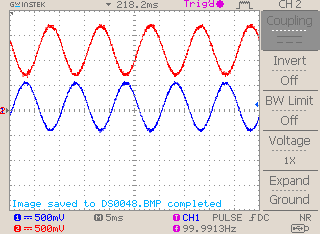
\includegraphics[width=1\textwidth]{../data/DS0049_n.png}
		\captionof{figure}{Amplification of a sine wave with a base voltage of \SI{1.5}{V}.}
		\label{fig:damp3}
	\end{Figure}

	At this point we were tasked to create a beat with two very slightly different frequencies. Since at this point we ran out of time, we were not able to do this. We are expecting to see the typical image of a beat, where two sine wave interfere with each other and produce a seemingly standing wave wich does not propergate. We would have used the normal frequency generator where we would set the variable frequency to the fixed frequency of another generator.
	\section{Conclusion}


	Afterwards we used an Adder to produce a sawtooth signal where our experimental optimum was slightly diffrent to the calculated one. We calculated for the \SI{150}{Hz} sine wave the best amplitude to be $\frac{1}{3}U_0$. We found that $\frac{1}{6}U_0$ was better in approximating the sawtooth signal.

	With the constant current source we showed that any resistor in the feedback loop had no influence in the current and the only way to modify it would be to change the voltage or resistance of the source.

	Proceeding, we build an intergrator wich integrated a square wave signal and found an frequency dependncy. Removing a resistor that should be parallel to the condesator showed fragmentations in the output. Switching to sine waves we oberseved the integration to a cosine and could produce, through varying the frequency and input voltage, a nearly perfect circel of a Lissajour figure.

	Lastly we build a differential amplifier, where we observed the shifting of the output through increasing the grounded positiv voltage. Because we had no time left, we could not create a beat, but the theory and outcome is fully understood.

	Overall the lab course was very successfull.

\end{multicols}


\clearpage
\listoffigures
\listoftables
\bibliographystyle{plain}
\bibliography{refs}

%}}}

\end{document}
